% =====================================================================
%  NeuroPilot - Complete System Flowchart (one page, TikZ)
%  ---------------------------------------------------------------------
%  HOW TO COMPILE
%    * Overleaf: new project -> upload this file -> compiler: pdfLaTeX.
%    * Local:    pdflatex NeuroPilot_Architecture.tex
%    * Needs only: standalone class, tikz, xcolor (all in TeX Live /
%      MiKTeX / Overleaf defaults). Output is a tightly-cropped vector
%      PDF - ideal for \includegraphics into a PPT slide or a paper.
%
%  To embed in an existing document instead, copy everything between
%  \begin{tikzpicture} ... \end{tikzpicture} (plus the \tikzset block
%  and \definecolor lines) into your preamble/body.
%
%  Geometry note: coordinates mirror the SVG original (x right, y DOWN)
%  via the negative y-unit trick, so px coordinates map 1:1
%  (1 px = 0.015 cm; canvas 1188 x 768 px = 17.8 x 11.5 cm).
% =====================================================================
\documentclass[tikz,border=10pt]{standalone}
\usepackage[T1]{fontenc}
\usepackage[utf8]{inputenc}
\usepackage{xcolor}
\usetikzlibrary{arrows.meta,positioning,calc,shapes.geometric}

% ---- palette (matches the NeuroPilot brand) ----
\definecolor{npink}{HTML}{16181B}   % ink
\definecolor{npwire}{HTML}{3F4654}  % default wire
\definecolor{npmut}{HTML}{5B6472}   % muted text
\definecolor{npfaint}{HTML}{6A7280} % zone labels
\definecolor{npzone}{HTML}{9AA0AB}  % zone stroke
\definecolor{npteal}{HTML}{0D8282}  % autonomous decision path
\definecolor{nppurple}{HTML}{7C3AED}% model feedback
\definecolor{npamber}{HTML}{B45309} % safety / audit / decisions
\definecolor{npgreen}{HTML}{0F766E} % live update path

\tikzset{
  % plain process box: sharp-ish corners, thin stroke, left-aligned text
  pbox/.style={
    draw=npink!75, fill=white, line width=0.5pt, rounded corners=2pt,
    align=left, anchor=north west, inner sep=3.2pt,
    font=\fontsize{6.4}{7.6}\selectfont,
  },
  ptitle/.style={font=\fontsize{7.3}{8.4}\selectfont\bfseries},
  % dashed zone container
  zone/.style={draw=npzone, dashed, line width=0.55pt, fill=white, fill opacity=0.35},
  zlabel/.style={font=\fontsize{6.4}{7.4}\selectfont\bfseries, text=npfaint},
  % decision diamond
  dec/.style={
    diamond, draw=npamber, fill=white, line width=0.6pt, align=center,
    inner sep=1.2pt, aspect=2.1,
    font=\fontsize{7.0}{8.0}\selectfont\bfseries,
  },
  % wires
  w/.style={->, line width=0.55pt, draw=npwire, >={Stealth[length=4.5pt]}},
  wt/.style={w, draw=npteal},
  wa/.style={w, draw=npamber, dashed},
  wp/.style={w, draw=nppurple, dashed},
  wg/.style={w, draw=npgreen, dashed},
  wl/.style={line width=0.55pt, draw=npwire},   % no arrow (bus segments)
  wlt/.style={line width=0.55pt, draw=npteal},
  % wire labels
  wlbl/.style={font=\fontsize{5.9}{6.8}\selectfont, text=npwire, inner sep=1pt},
  wlblt/.style={wlbl, text=npteal},
  wlbla/.style={wlbl, text=npamber},
  wlblp/.style={wlbl, text=nppurple},
  % mono
  mono/.style={font=\fontsize{5.8}{6.9}\selectfont\ttfamily},
}

\begin{document}
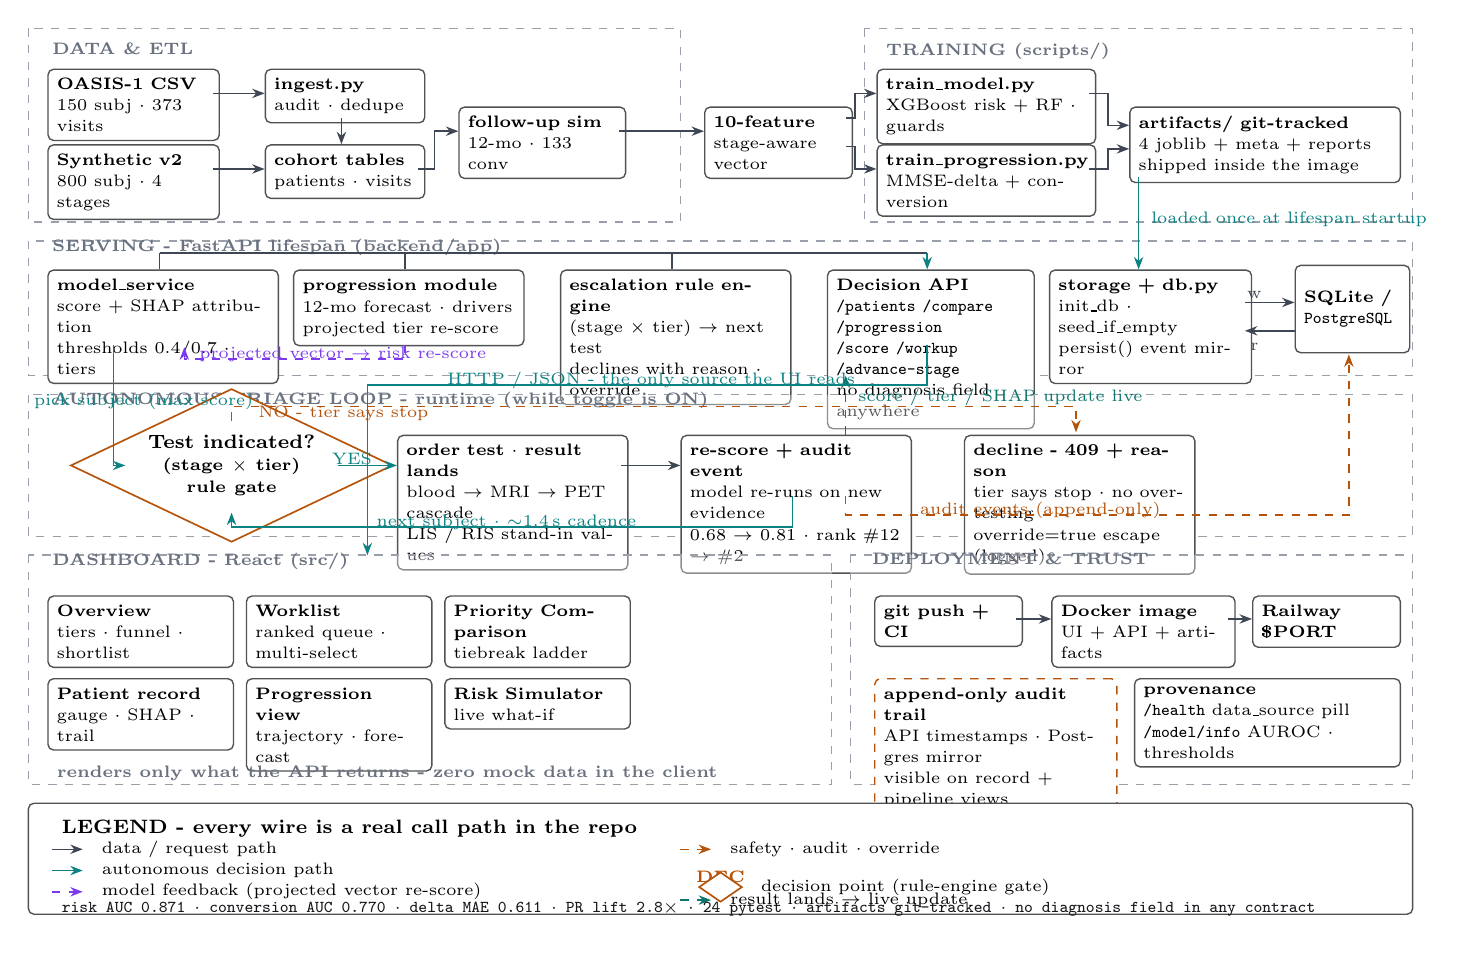
\begin{tikzpicture}[x=0.015cm, y=-0.015cm] % y grows DOWN like the SVG original

% =====================================================================
% BAND 1 - DATA & ETL  +  TRAINING  (y 6..170)
% =====================================================================
\draw[zone] (8,6) rectangle (560,170);
\node[zlabel, anchor=north west] at (20,10) {DATA \& ETL};

\node[pbox, minimum width=2.10cm, minimum height=0.63cm, text width=1.95cm] at (24,40)
  {\textbf{OASIS-1 CSV}\\ 150 subj $\cdot$ 373 visits};
\node[pbox, minimum width=2.10cm, minimum height=0.63cm, text width=1.95cm] at (24,104)
  {\textbf{Synthetic v2}\\ 800 subj $\cdot$ 4 stages};
\node[pbox, minimum width=1.95cm, minimum height=0.63cm, text width=1.80cm] at (208,40)
  {\textbf{ingest.py}\\ audit $\cdot$ dedupe};
\node[pbox, minimum width=1.95cm, minimum height=0.63cm, text width=1.80cm] at (208,104)
  {\textbf{cohort tables}\\ patients $\cdot$ visits};
\node[pbox, minimum width=2.04cm, minimum height=0.63cm, text width=1.89cm] at (372,72)
  {\textbf{follow-up sim}\\ 12-mo $\cdot$ 133 conv};
\node[pbox, minimum width=1.80cm, minimum height=0.72cm, text width=1.65cm] at (580,72)
  {\textbf{10-feature}\\ stage-aware vector};

\draw[w] (164,61) -- (208,61);
\draw[w] (164,125) -- (208,125);
\draw[w] (273,82) -- (273,104);
\draw[w] (338,125) -- (352,125) -- (352,93) -- (372,93);
\draw[w] (508,93) -- (580,93);

\draw[zone] (716,6) rectangle (1180,170);
\node[zlabel, anchor=north west] at (726,10) {TRAINING (scripts/)};

\node[pbox, minimum width=2.70cm, minimum height=0.63cm, text width=2.55cm] at (726,40)
  {\textbf{train\_model.py}\\ XGBoost risk + RF $\cdot$ guards};
\node[pbox, minimum width=2.70cm, minimum height=0.63cm, text width=2.55cm] at (726,104)
  {\textbf{train\_progression.py}\\ MMSE-delta + conversion};
\node[pbox, minimum width=3.36cm, minimum height=0.90cm, text width=3.21cm] at (940,72)
  {\textbf{artifacts/ git-tracked}\\ 4 joblib + meta + reports\\ shipped inside the image};

\draw[w] (700,82) -- (708,82) -- (708,61) -- (726,61);
\draw[w] (700,106) -- (708,106) -- (708,125) -- (726,125);
\draw[w] (906,61) -- (922,61) -- (922,88) -- (940,88);
\draw[w] (906,125) -- (922,125) -- (922,108) -- (940,108);

% =====================================================================
% BAND 2 - SERVING  (y 186..300)
% =====================================================================
\draw[zone] (8,186) rectangle (1180,300);
\node[zlabel, anchor=north west] at (20,176) {SERVING - FastAPI lifespan (backend/app)};

\node[pbox, minimum width=2.85cm, minimum height=0.96cm, text width=2.70cm] at (24,210)
  {\textbf{model\_service}\\ score + SHAP attribution\\ thresholds 0.4/0.7 $\cdot$ tiers};
\node[pbox, minimum width=2.85cm, minimum height=0.96cm, text width=2.70cm] at (232,210)
  {\textbf{progression module}\\ 12-mo forecast $\cdot$ drivers\\ projected tier re-score};
\node[pbox, minimum width=2.85cm, minimum height=0.96cm, text width=2.70cm] at (458,210)
  {\textbf{escalation rule engine}\\ (stage $\times$ tier) $\rightarrow$ next test\\ declines with reason $\cdot$ override};
\node[pbox, minimum width=2.55cm, minimum height=0.96cm, text width=2.40cm] at (684,210)
  {\textbf{Decision API}\\ {\ttfamily\fontsize{5.8}{6.9}\selectfont /patients /compare /progression}\\
   {\ttfamily\fontsize{5.8}{6.9}\selectfont /score /workup /advance-stage}\\ no diagnosis field anywhere};
\node[pbox, minimum width=2.49cm, minimum height=0.96cm, text width=2.34cm] at (872,210)
  {\textbf{storage + db.py}\\ init\_db $\cdot$ seed\_if\_empty\\ persist() event mirror};
\node[pbox, minimum width=1.38cm, minimum height=1.11cm, text width=1.23cm] at (1080,206)
  {\textbf{SQLite /}\\ {\ttfamily PostgreSQL}};

% API bus above the serving boxes
\draw[wl]  (119,210) -- (119,196);
\draw[wl]  (327,210) -- (327,196);
\draw[wl]  (553,210) -- (553,196);
\draw[wl]  (119,196) -- (769,196);
\draw[wt]  (769,196) -- (769,210);

% artifacts loaded once at startup
\draw[wt] (948,132) -- (948,210);
\node[wlblt, anchor=west] at (956,168) {loaded once at lifespan startup};

% DB read/write
\draw[w]  (1038,238) -- (1080,238);
\node[wlbl] at (1046,232) {w};
\draw[w]  (1080,262) -- (1038,262);
\node[wlbl] at (1046,276) {r};

% feedback: progression -> risk model re-score (dashed purple)
\draw[wp] (327,274) -- (327,286) -- (140,286) -- (140,276);
\node[wlblp, anchor=west] at (150,282) {projected vector $\rightarrow$ risk re-score};

% =====================================================================
% BAND 3 - AUTONOMOUS TRIAGE LOOP  (y 316..436)
% =====================================================================
\draw[zone] (8,316) rectangle (1180,436);
\node[zlabel, anchor=north west] at (20,306) {AUTONOMOUS TRIAGE LOOP - runtime (while toggle is ON)};

\node[dec, minimum width=2.70cm, minimum height=1.14cm, text width=2.2cm] at (180,376)
  {Test indicated?\\ {\fontsize{5.8}{6.8}\selectfont (stage $\times$ tier) rule gate}};
\node[pbox, minimum width=2.85cm, minimum height=0.78cm, text width=2.70cm] at (320,350)
  {\textbf{order test $\cdot$ result lands}\\ blood $\rightarrow$ MRI $\rightarrow$ PET cascade\\ LIS / RIS stand-in values};
\node[pbox, minimum width=2.85cm, minimum height=0.78cm, text width=2.70cm] at (560,350)
  {\textbf{re-score + audit event}\\ model re-runs on new evidence\\ 0.68 $\rightarrow$ 0.81 $\cdot$ rank \#12 $\rightarrow$ \#2};
\node[pbox, minimum width=2.85cm, minimum height=0.78cm, text width=2.70cm] at (800,350)
  {\textbf{decline - 409 + reason}\\ tier says stop $\cdot$ no over-testing\\ override=true escape (logged)};

\draw[wt] (80,274) -- (80,376) -- (90,376);
\node[wlblt, anchor=west] at (10,322) {pick subject (max score)};
\draw[wt] (270,376) -- (320,376);
\node[wlblt] at (282,370) {YES};
\draw[w]  (510,376) -- (560,376);
\draw[wt] (655,402) -- (655,428) -- (180,428) -- (180,416);
\node[wlblt, anchor=west] at (300,424) {next subject $\cdot$ $\sim$1.4\,s cadence};
\draw[wa] (180,338) -- (180,326) -- (895,326) -- (895,348);
\node[wlbla, anchor=west] at (200,332) {NO - tier says stop};
\draw[wg] (700,350) -- (700,300);
\node[wlbl, anchor=west, text=npgreen] at (708,318) {score / tier / SHAP update live};
\draw[wa] (700,402) -- (700,418) -- (1126,418) -- (1126,282);
\node[wlbla, anchor=west] at (760,414) {audit events (append-only)};

% =====================================================================
% BAND 4 - DASHBOARD  +  DEPLOYMENT & TRUST  (y 452..646)
% =====================================================================
\draw[zone] (8,452) rectangle (688,646);
\node[zlabel, anchor=north west] at (20,442) {DASHBOARD - React (src/)};

\node[pbox, minimum width=2.28cm, minimum height=0.63cm, text width=2.13cm] at (24,486)
  {\textbf{Overview}\\ tiers $\cdot$ funnel $\cdot$ shortlist};
\node[pbox, minimum width=2.28cm, minimum height=0.63cm, text width=2.13cm] at (192,486)
  {\textbf{Worklist}\\ ranked queue $\cdot$ multi-select};
\node[pbox, minimum width=2.28cm, minimum height=0.63cm, text width=2.13cm] at (360,486)
  {\textbf{Priority Comparison}\\ tiebreak ladder};
\node[pbox, minimum width=2.28cm, minimum height=0.63cm, text width=2.13cm] at (24,556)
  {\textbf{Patient record}\\ gauge $\cdot$ SHAP $\cdot$ trail};
\node[pbox, minimum width=2.28cm, minimum height=0.63cm, text width=2.13cm] at (192,556)
  {\textbf{Progression view}\\ trajectory $\cdot$ forecast};
\node[pbox, minimum width=2.28cm, minimum height=0.63cm, text width=2.13cm] at (360,556)
  {\textbf{Risk Simulator}\\ live what-if};
\node[zlabel, anchor=north west] at (24,622)
  {renders only what the API returns - zero mock data in the client};

\draw[wt] (769,274) -- (769,308) -- (295,308) -- (295,452);
\node[wlblt, anchor=west] at (360,304) {HTTP / JSON - the only source the UI reads};

\draw[zone] (704,452) rectangle (1180,646);
\node[zlabel, anchor=north west] at (714,442) {DEPLOYMENT \& TRUST};

\node[pbox, minimum width=1.80cm, minimum height=0.60cm, text width=1.65cm] at (724,486)
  {\textbf{git push + CI}};
\node[pbox, minimum width=2.25cm, minimum height=0.60cm, text width=2.10cm] at (874,486)
  {\textbf{Docker image}\\ UI + API + artifacts};
\node[pbox, minimum width=1.80cm, minimum height=0.60cm, text width=1.65cm] at (1044,486)
  {\textbf{Railway \$PORT}};
\draw[w] (844,506) -- (874,506);
\draw[w] (1024,506) -- (1044,506);

\node[pbox, minimum width=3.00cm, minimum height=0.90cm, text width=2.85cm,
      draw=npamber, dashed] at (724,556)
  {\textbf{append-only audit trail}\\ API timestamps $\cdot$ Postgres mirror\\ visible on record + pipeline views};
\node[pbox, minimum width=3.30cm, minimum height=0.90cm, text width=3.15cm] at (944,556)
  {\textbf{provenance}\\ {\ttfamily /health} data\_source pill\\ {\ttfamily /model/info} AUROC $\cdot$ thresholds};

% =====================================================================
% BAND 5 - LEGEND  (y 662..756)
% =====================================================================
\draw[draw=npink!75, fill=white, line width=0.5pt, rounded corners=2pt] (8,662) rectangle (1180,756);
\node[anchor=north west, font=\fontsize{7.0}{8.0}\selectfont\bfseries] at (28,668)
  {LEGEND - every wire is a real call path in the repo};

\draw[w]  (28,701) -- (54,701);  \node[anchor=west, font=\fontsize{6.4}{7.4}\selectfont] at (62,701) {data / request path};
\draw[wt] (28,719) -- (54,719);  \node[anchor=west, font=\fontsize{6.4}{7.4}\selectfont] at (62,719) {autonomous decision path};
\draw[wp] (28,737) -- (54,737);  \node[anchor=west, font=\fontsize{6.4}{7.4}\selectfont] at (62,737) {model feedback (projected vector re-score)};
\draw[wa] (560,701) -- (586,701);\node[anchor=west, font=\fontsize{6.4}{7.4}\selectfont] at (594,701) {safety $\cdot$ audit $\cdot$ override};
\node[font=\fontsize{5.6}{6.4}\selectfont\bfseries, text=npamber] at (594,724) {DEC};
\node[dec, minimum width=0.55cm, minimum height=0.38cm, inner sep=0.5pt] at (594,733) {};
\node[anchor=west, font=\fontsize{6.4}{7.4}\selectfont] at (620,733) {decision point (rule-engine gate)};
\draw[wg] (560,744) -- (586,744);\node[anchor=west, font=\fontsize{6.4}{7.4}\selectfont] at (594,744) {result lands $\rightarrow$ live update};

\node[anchor=west, mono, text=npink] at (28,752)
  {risk AUC 0.871 $\cdot$ conversion AUC 0.770 $\cdot$ delta MAE 0.611 $\cdot$ PR lift 2.8$\times$ $\cdot$ 24 pytest $\cdot$ artifacts git-tracked $\cdot$ no diagnosis field in any contract};

\end{tikzpicture}
\end{document}
